\documentclass[11pt]{report}
    \usepackage[french]{babel}
    \usepackage[utf8]{inputenc}
    \usepackage[T1]{fontenc} 
    \usepackage{graphicx}
    \usepackage{tikz}
    \usepackage{tocbibind}
    \usepackage[pdftex,colorlinks=true,linkcolor=blue,citecolor=blue,urlcolor=blue]{hyperref}
    \usepackage{anysize}
    \usepackage{icomma}
    \usepackage[pagestyles]{titlesec}
    \usepackage{titlesec}
    \usepackage{glossaries}
    
    % marges
    \usepackage[margin=2cm]{geometry}
    % Font (calibri like)
    % Line spacing
    \usepackage{setspace}


    \usetikzlibrary{positioning}
    \DeclareGraphicsExtensions{.jpg,.pdf,.png,.PNG}
    \fboxsep=0mm%padding thickness
    \fboxrule=1pt%border thickness
    % Chapters titles
    \titleformat{\chapter}[block]{\Large\bfseries}{\thechapter}{1em}{}
    \titleformat{\section}[block]{\large\bfseries}{\thesection}{1em}{}
    \titleformat{\subsection}[block]{\bfseries}{\thesubsection}{1em}{}
    % Delete some spaces between the chapter title and the top of the page
    \titlespacing*{\chapter}{0pt}{-20pt}{20pt}
    
    \makeglossaries
    \loadglsentries{Pages/Glossaire}
    \begin{document}
    \begin{titlepage}
        \begin{tikzpicture}[overlay, remember picture]
            \path (current page.north east) ++(-1,-1) node[below left] {FELIX Alexandre, Architecture des logiciels, Promotion 2017-2018};
        \end{tikzpicture}
    \begin{center} 
    \begin{figure}
        \centering
        \begin{minipage}{0.33\textwidth}
            
\includegraphics[width=0.8\textwidth]{Images/eurice} % Entreprise
        \end{minipage}
        \begin{minipage}{0.33\textwidth}
            \centering
            
\includegraphics[width=0.8\textwidth]{Images/esgi} % École
        \end{minipage}
    \end{figure}
    ~\\[3\baselineskip]
    
    % Title
    \rule{\linewidth}{0.5mm} \\[0.4cm]
    { \huge \bfseries Rapport d'activité en entreprise\\[0.4cm] }
    \rule{\linewidth}{0.5mm} \\[1.5cm]
    
    % Supervisors
    {\large Entreprise: Eurice}\\[0.3cm]
    {\large Tuteur en entreprise: Yannick Lavoix (Eurice)}\\[0.3cm]
    {\large Septembre 2017 - Septembre 2019, Contrat de professionalisation}\\[0.3cm]
    \vfill
    % Bottom of the page
    \end{center}
    \end{titlepage}
    \clearpage
    
    \chapter*{Remerciements}
    \addcontentsline{toc}{chapter}{Remerciements}
    Tout d’abord, je remercie M. Yannick Lavoix, mon maître d’apprentissage,
    pour m’avoir encadré durant cette alternance. 
    
    
    Je souhaite remercier l’ensemble de l’entreprise Eurice qui a
    rendu cet apprentissage possible et m’a permis d’acquérir de nombreux nouveaux
    savoirs et compétences.\newline
    
    Enfin, je remercie l'ESGI pour avoir rendu
    cette alternance possible et m’avoir fait bénéficier de cours enrichissants avec
    une équipe pédagogique de qualité tout au long de l’année. \newline

    \renewcommand{\baselinestretch}{1.30}\small \normalsize
    \tableofcontents
    \renewcommand{\baselinestretch}{1.18}\small \normalsize
    
    \chapter*{Introduction}
\addcontentsline{toc}{chapter}{Introduction}
Dans le cadre de ma 5ième année d'architectures des logiciels en apprentissage, 
je devais intégrer une entreprise, j'ai continué cette année l'alternance que j'avais commencé 
dans l'entreprise Eurice pendant ma 4ième année.\newline

%objectif du présent stage
Le but de cette alternance est de nous confronter au monde professionnel, 
d’acquérir une expérience en entreprise et enfin communiquer notre ressenti et 
notre travail effectué en entreprise à travers la rédaction de ce rapport. \newline

%Missions effectuées
Eurice fourni des solutions logiciel pour les centres d'appel 
que ce soit pour l'accueil téléphonique ou la gestion d'agenda. 
Je travaille au sein de l’équipe de développement. 

Mes missions pendant ces 12 mois ont été de continuer le développement de l'application mobile pour la gestion d'agenda
dont j'ai commencé le développement en 4ième année et avaner dans le développement de la nouvelle version du site client . \newline

%Structure du rapport
Dans une première grande partie je présenterai l’entreprise. 
Dans une seconde partie je ferai une introduction des logiciels réalisés à Eurice, 
nécessaire pour comprendre le contexte de ma mission 
puis je présenterai ma mission et les différentes tâches effectuées.
Dans une troisième partie, j'expliquerai l'apport de mon cursus professionnel et scolaire à mon accomplissement
en tant qu'ingénieur informatique pour finir par une conclusion \newline



    \chapter{Contexte Entreprise}
\section{Entreprise d'accueil}
L’accueil téléphonique en France est principalement utilisé par les professions libérales 
mais également pour les entreprises de toutes tailles souhaitant avoir un accueil téléphonique.
Cette profession dispose de sa chambre professionnelle  le « SIST » qui regroupe 60 centres d’accueil partout en France cela représente 
8000 hôtesses d'accueil téléphonique et 150 millions d'appels entrant traités par an. 
Le principe de l’accueil téléphonique est de ne rater aucun appel téléphonique 
pour ne pas perdre de potentiel client. \newline

Le fait de confier sa ligne téléphonique à des professionnels 
permet d’avoir un accueil téléphonique de qualité et permet également de réduire drastiquement les coûts qu’aurait une entreprise à engager 
une ou plusieurs personnes à temps plein pour répondre aux appels.\newline

Créée en 1992 par ses actuels dirigeants, Eurice est spécialisée dans la gestion d'appels entrants 
et est à la fois opérateur et fournisseur de solutions techniques de par ses services:
\begin{itemize}
	\item L'accueil téléphonique fourni par un plateau de réception des appels 
	au sein des locaux de l'entreprise, qui peut aussi parfois servir d’environnement de pré-production 
	avant le déploiement de mise à jour chez les centres d'appels client.

	\item Le développement de solutions pour les centres d'appels: logiciel de gestion d'agenda, 
	répartiteur d'appel, portail client et applications mobiles, tous les logiciels utilisés à Eurice 
	et vendus au client, cela permet entre autre de connaître le besoin avec plus de précision 
	car nous sommes clients de nos propres produits.
\end{itemize}
Chaque année, Eurice gère pour le compte de ses clients près 
d'un million d'appels décrochés en moins de 3 sonneries.

\begin{figure}[h]
	\centering
	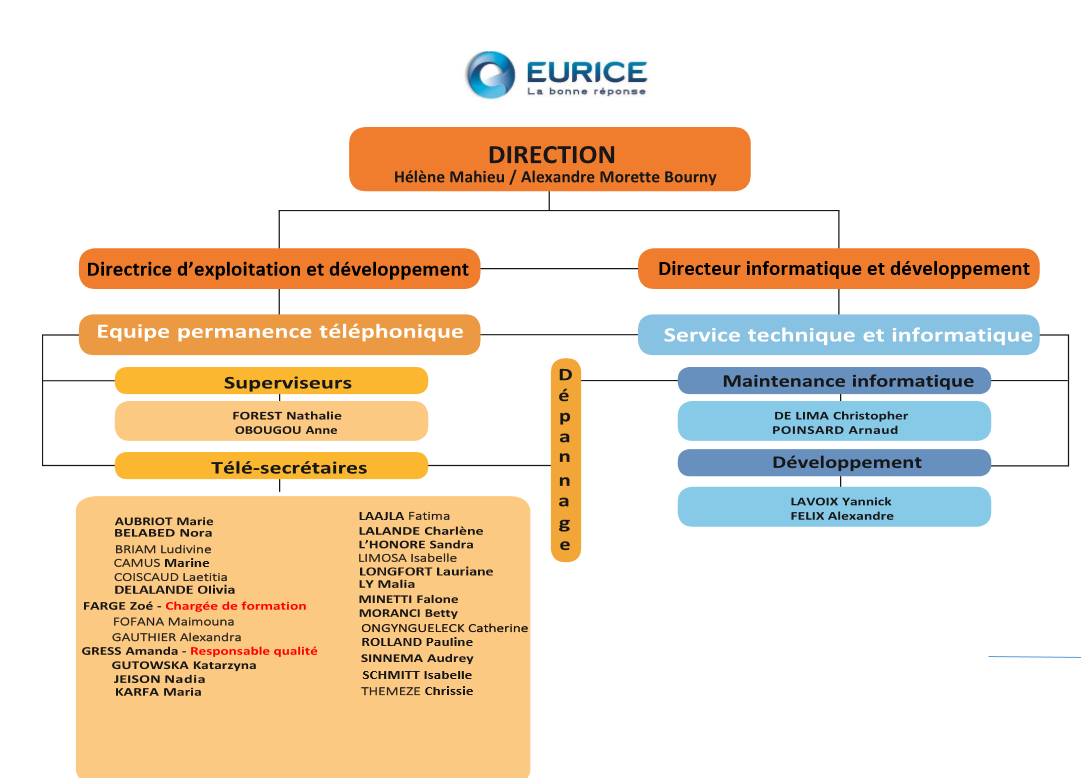
\includegraphics[width=0.7\linewidth]{Images/organigramme_fonctionnel}
	\caption{Organigramme Fonctionnel}
	\label{fig:organigrammefonctionnel}
\end{figure}

\section{Contexte Métier}

\subsection{Callibri}
Il s'agit de l'application principale pour un centre d'appel. 
Ce logiciel permet la gestion de plusieurs dossiers avec leur agenda, 
avoir une communication entre la secrétaire et le client via les instructions et les messages. 
un système de scripting soutient l'opératrice lors du traitement d'un appel, 
c'est le support du pré-traitement et du post-traitement de l'appel. \newline

\gls{Callibri} s'interface avec le système d'appel pour automatiquement ouvrir le dossier correspondant 
au numéro appelé, cela permet de gagner un temps conséquent 
et de rendre transparent l'appel au yeux de l'appelant qui ne sait pas 
que son appel est décroché dans un centre d'appel. \newline


L'application utilise pour la majeure partie de l'interface des pages web grâce 
à la librairie Essentials Objects utilisant un moteur chrome embarqué.
Le reste de l'interface qui comprend le menu et la fenêtre native est réalisé en WPF.
\newline


\gls{Callibri} étant utilisé sur plusieurs postes accédant à des ressources communes, 
le logiciel communique via messages UDP aux autres postes, pour, par exemple, éviter de prendre 
un rendez-vous sur le même créneau libre.

\section{Focus sur le service du stage}
Je fais partie de l'équipe développement qui est composé de Yannick Lavoix et de moi-même, 
notre objectif est d'ajouter des fonctionnalités aux logiciels existant, 
les maintenir et créer de nouvelles solutions. notre interlocuteur principal est le directeur
de l'entreprise Mr. Morette-Bourny, nous sommes parfois mis en relation avec des clients 
ou des partenaires tel que RDVMedicaux ou Doctolib. \newline

\subsection{Site Client "Web2"}
le site client, portant le dénomination web2, permet l'accès aux 
clients finaux (practiciens dans le médical principalement) à leurs agenda,
il a été développé an ASP.Net 4.5 avec un front-end html + css + js avec jquery.
ce projet peut être considéré comme ayant du code legacy car il n'y a aucun 
test unitaires, aucune documentation et le code ne respecte pas la majorité
des principes basiques de la programmation orienté objet.

\subsection{Callibri Mobile}
Callibri Mobile est l'application android et iOS qui permet aux clients finaux 
d'acceder à leur agenda depuis leur téléphone, il ne s'agit pas d'une version 
responsive du web2 utilisé pas un wrapper pour faire une application mais bien
une application indépendantes et optimisé pour l'expérience smartphone,
il s'agit du projet principal de mes 2 années d'alternance. 



    \chapter{Mission Principale}
Ma mission lors de cette 5ième année a été de continuer le développement de l'application mobile Callibri Mobile
que j'ai commencé vers le milieu de la 4ième année, cette application est la refonte complète de l'ancienne 
application mobile qui n'est qu'un wrapper de navigateur autour du site web2 en responsive,
aujourd'hui les application mobiles étant un passage obligatoire pour fournir aux clients une experience 
correcte d'utilisation de nos services et pour rester compétitif face à nos concurrent 
il était nécéssaire de réaliser une application qui soit pensé pour une interface de smartphone et 
non juste une adaptation. \newline

lors de la 4ième année je me suis familiarisé avec Ionic et Angular, les deux framework que j'ai utilisé pour 
le développement de l'application, Ionic est un framework qui permet de créer des application mobile 
iOS et Android mais aussi desktop via electron en utilisant des technologies web.\newline

Au début du développement Ionic n'était qu'à ses balbutiements avec la version 1.3 et utilisait uniquement 
le framework angular, j'ai du très tôt dans le cycle de déveleppement porter la version vers ionic 2 qui n'etait pas retro 
compatible.\newline

Lors de ma 5ième année Ionic a subis de nombreux changements, le plus notable étant le changement de la version 3 
à la version 4, ce dernier est devenu framework-agnostic c'est à dire qu'il ne dépend plus d'un framework 
web sousdjacent spécifique mais peut être utilisé par les autres framework web les plus connus tel que 
React et vuejs mais aussi en standalone avec du javascript pure. \newline 

Comme nous avant passé plus d'un an à développer l'application en utilisant le framework Angular nous 
avons décider de continuer ce qui n'a pas empecher le fait que le changement de version 
a entrainé de nombreux changement qui fut le but principal de ma mission de 5ieme année. \newline

En passant à sa version 4, Ionic apporte grand nombre de changement:

\begin{itemize}
	\item passage d'angular 2+ à angular 7+: un grand bon en avant en terme de performance, ce qui 
	est très rechercher pour le développement hybride d'application mobile car cela permet de reduire 
	la différence de fluidité avec une application native. \newline

	\item utilisation du router angular en lieu et place du navcontroller de ionic:
	l'équipe de développement de Ionic à decider de permettre d'utiliser le meilleur 
	de chaquer framework du stack et le routeur angular en fait partie, cela fut une 
	partie assez difficile à mettre correctement en place car l'application 
	callibri mobile à une grande quantité de page et de modales. \newline 

	\item apparition du shadow-dom: un nouveau système utilisé dans le rendu du DOM,
	le shadow DOM est comme un subtree du DOM, il permet notammenet de simplifier 
	le fonctionnement des règles CSS mais surtout d'augmenter les performance de rendu 
	de l'html qui sont loin d'être optimales dans le cas d'un smartphone. \newline
	\begin{figure}[!h]
		\centering
		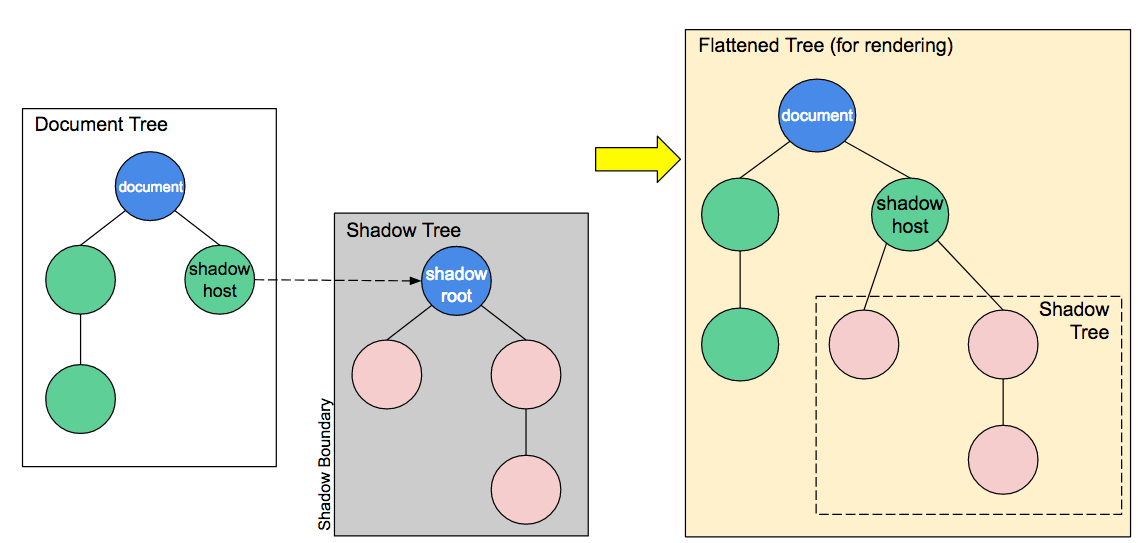
\includegraphics[width=1\linewidth]{Images/shadow}
		\caption{fonctionnement du shadow dom}
		\label{fig:archhexa}
	\end{figure}

	\item De nombreux changement dans le fonctionnement des composants Ionic et de leur 
	syntax ce qui a du nécéssiter la réecriture d'une bonne partie des fichiers html 
	de l'application plus un changement de l'architecture des fichiers du projet 
	pour refleter ces divers changement. \newline
\end{itemize}

Tout ces changments ont aussi été l'occasion de perfectionner le look de l'application 
et l'intuitivité de ses interfaces, le fastmenu qui etait un menu d'accès rapide sous 
forme de cercle disponible sur toutes les pages de l'application a été supprimé,
il prenait beaucoup de place inutilement pour être une duplication des contrôles 
déjà disponibles. \newline 

\section{Agenda}
Ce fut la partie de l'application qui a subis le plus de changement, anciennement l'agenda 
utilisait du code de très mauvaise qualité pour répondre à un besoin technique presque inexistant.
l'agenda utilise deux vues: la vue jour et la vue mois, dans l'ancienne version majeure
de l'application un système de cache complexe était utilisé pour charger une semaine entière 
et ainsi ne pas avoir à faire des appel regulier au serveur, pour l'affichage 
un système de slide tout aussi complexe était utilisé pour faire correspondre le jour affiché 
avec un des 7 jours en cache, cet ensemble était très mal écrit, tout à fait intestable 
et peu performant. \newline

pendant ma 5ième année j'ai refait cette page agenda, qui est la page la plus importante 
de tout l'application, en supprimant ce système de cache qui était plus source d'erreur 
et de difficulté de maintenabilité qu'autre chose puisqu'au final la requête pour charger 
un jour de l'agenda depuis le serveur est très simple et rapide. \newline

nous avons supprimer le système de slide par un système simple d'animation in \& out css 
qui donne l'impression que la page part sur le côté de l'écran pour laisser la page suivante
arriver du côté opposé, en plus de performance multiplié par un facteur 10, le code à été 
fortement réduit, l'animation est utilisé pour cacher une partie du chargement de la
nouvelle journée de l'agenda. \newline

\begin{figure}[!h]
	\centering
	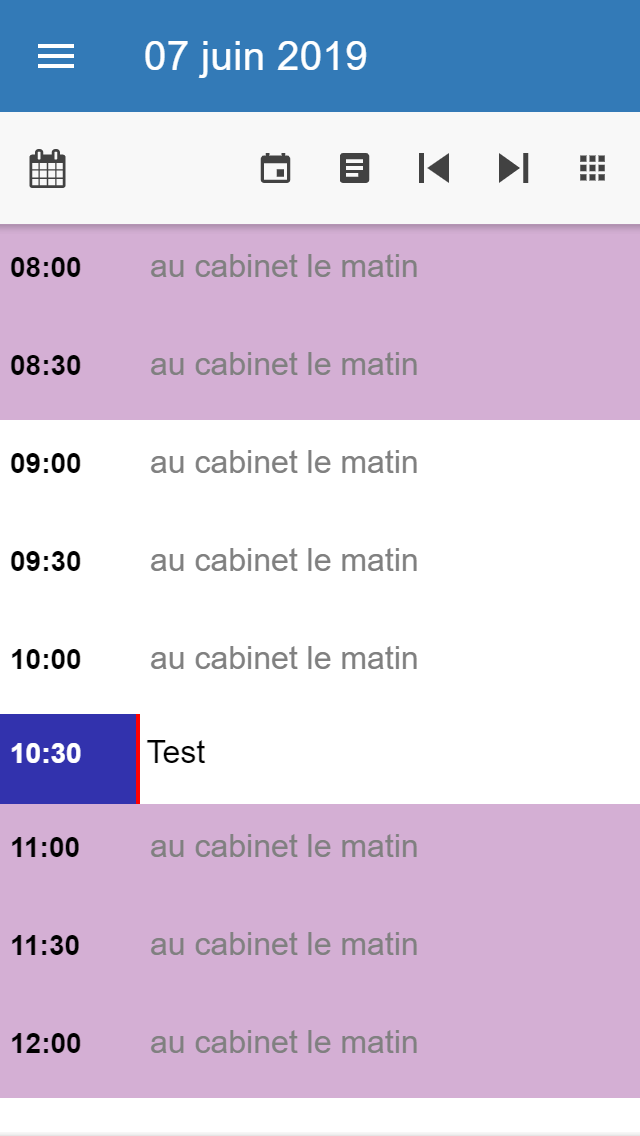
\includegraphics[width=0.3\linewidth]{Images/agenda}
	\caption{les changements visuels de la page agenda son mineur et ne deroutent pas l'utilisateur }
	\label{fig:archhexa}
\end{figure}

\section{Contact}

la page de contact a subis de nombreux changements aussi mais plus du côté du code 
que l'interface graphique, le système de recherche de contact à été optimisé du côté 
du serveur pour ainsi avoir une latence de réponse plus faible et des résultats 
avec moins d'erreurs, l'affichage de la page de recherche est plus fluide car j'ai 
changé l'architecture des données pour utilisé de manière plus poussée le reactive 
programming et avoir l'état de l'interface graphique qui change correctement en 
fonction des données ce qui parfois n'était pas le cas avec l'ancienne version 
ou une mauvaise synchronisation entre par exemple le spinner de chargement 
et le chargement des données était differé de plusieurs centaines de millisecondes 
ce qui a un impact conséquent sur l'impression de fluidité. \newline

Le transfert d'information et de contact entre les différentes pages utilisant un contact tel
que la liste de contact, l'ajout de contact et la selection de contact depuis l'ajout 
d'un rendez-vous dans l'agenda à été réduite à son minimum pour simplifier le tracage 
des état de l'application: auparavant la liste de contact envoyait l'id du contact 	
à la page de details du contact qui chargeait les informations du contact et en cas de modification 
du contact renvoyait une commande à la page qui executait la commande qui consistait 
en un appel http pour modifier le contact puis le mettre à jour dans la liste de contacts.
\newline

J'ai refactorisé le code et notamment transformé de nombreuses pages en modales y compris la page
des détails d'un contact, dans la version actuelle de l'application la page liste de contact 
ouvre une modales avec l'id du contact et lors de modifications c'est la modale
elle même qui fait des appels http, la modale retourne un resultat vide lors de sa fermeture 
ou un objet contact si des modifications ont été faites pour pouvoir mettre à jour la liste, 
ce fonctionnement de type master-details est aussi présent pour les instructions, les messages 
et l'agenda et ce comportement y a été reproduit de la même manière dans ces dernières. 

\begin{figure}[!h]
	\centering
	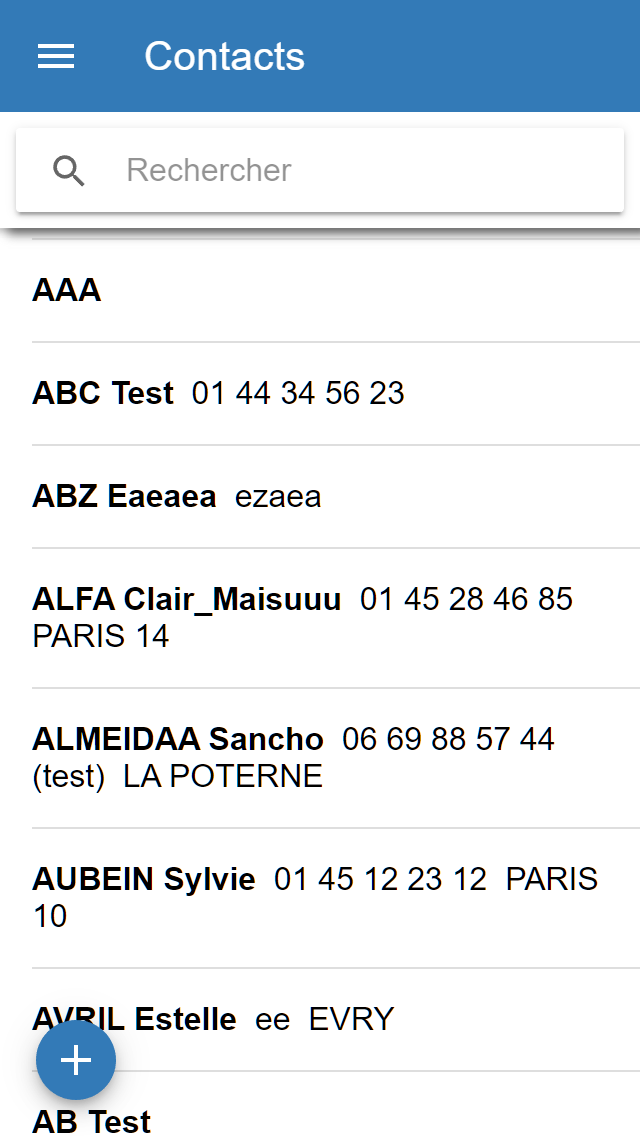
\includegraphics[width=0.35\linewidth]{Images/contact}
	\caption{Page des contacts}
	\label{fig:archhexa}
\end{figure}



\newpage
\section{Bilan et recul sur la mission}
Pour cette mission j'ai eu totale liberté dans mes choix qui fut à la fois un avantage mais 
aussi une preuve du manque de gestion de projet au sein de l'entreprise, je n'avais 
aucun cahier des charges et les règles métiers n'etaient pas clairement définies,
j'ai du donc établir par moi même le cahier des charge et lister les nouvelles fonctionnalitées 
en me basant sur l'ancien site web et son code qui n'a d'ailleurs pas facilité la tache. \newline

j'ai du aussi me baser sur le website et m'auto-former aux bonnes pratiques 
à appliquer à l'expérience utilisateur et l'interface graphique puisqu'une application
n'a pas du tout les mêmes contraintes qu'un site web. \newline

Lors de mon rapport de 4ième année j'avais tiré la conclusion que javascript et son 
écosystème est assez médiocre en terme de qualité des outils et framework, 
un an plus tard mon avis a un peu changé, je pense qu'il est possible de trouver 
des framework de qualité, comme Ionic avec sa dernière version, Angular ou React 
et je pense finalement avoir fait les bon choix technologique pour cette application 
pour le long terme mais malgré cela je ne pense pas que javascript serait mon premier 
choix pour autre chose que du web.
 \newline





    \include{Pages/Conclusion}
    \chapter{Le Métier d'ingénieur informatique}
L'ingénieur informatique est un professionnel appliquant les principes de l'ingénieurie au développement de logiciels,
il possède de nombreuses compétences n'appartenant pas au seul domaine de la programmation tel que les bonnes pratiques 
(extreme programming, KISS, SOLID), connaissances approfondies de l'algorithmie, des structures de données 
et de la scalablilité, le tout associé à une veille technologique regulière pour toujours savoir
repondre au besoin de manière pertinente.

\section{Apport de mon parcours}
\subsection{Alternance}
L'alternance pendant ma 4ième année m'a apporté beaucoup de compétence en développement avec l'apprentissage 
du framework angular, ionic et asp.net 
j'ai forgé des compétences en web qui était quasiment inexistante auparavant car je n'avais fait que 
du développement d'application de bureau pendant mes stages en BTS, comprendre plusieurs paradigme 
et plusieurs types de stack technologiques (web, mobile, desktopp) est très important pour ingénieur
qui doit avoir une multitude d'outils technologiques à sa ceinture \newline

Lors de la 5ième année je suis rapidement arrivé au bout de ce que pouvais m'offrir l'entreprise en  
terme d'acquisition de compétences, en effet l'entreprise ou j'ai fait mon alternance 
n'a pas une taille permettant de recruter une équipe d'ingénieurs et dans une équipe 
de 2 personnes difficile d'apprendre l'importance de communiquer ou les compétences en 
communication essentielles pour un ingénieur. \newline

Une autre problématique s'est posé lors de ma 5ième année qui fut à la fois un frein et bénefique pour 
mes compétences mais uniquement grâce à ma curiosité intellectuelle et mon envie de me surpasser là dans ce quoi 
je suis compétent, il s'agit de la qualité abyssale des projet sur lequels j'ai été amené à travailler 
en dehors de ma mission principale. En effet la qualité du code est quasi-nulle, aucun test unitaires, les principes 
considérés comme primordial de la programmation tel que SOLID ou KISS ne sont pas respectés, ni le paradigme 
même des langages utilisés. \newline

Travailler sur un code qui est de niveau, tout au plus, débutant associé à l'absence de toute 
gestion de projet ne permet pas d'acquérir des compétences via un acteur exterieur, 
l'effet insoupçonné est que j'ai appris a reconnaître avec beaucoup plus de rapidité 
et de pragmatisme les défaut de l'architecture d'un logiciel, de plus j'ai appris 
de façon très poussé la refactorisation de code et comment trouver les "code smells" pour 
les corriger. J'ai aussi fait une veille technologique journalière poussé sur l'architecture 
et les bonnes pratiques pour pouvoir l'appliquer sur ma mission principale et 
les projets où je pouvais faire des modifications retro-compatibles. 


\newpage

\subsection{Parcours Scolaire}


\subsection{Ce qui fait de moi un bon ingénieur}

\section{Projet professionnel}
Mon projet professionnel est déjà lancé puisque j'ai déjà signé mon CDI chez SOAT une 
société de conseil dans laquelle je vais être ingénieur d'etudes, je souhaite évoluer 
au sein de cette entreprise et monter le plus rapidement possible en compétence technique 
mais aussi surtout dans le management et les méthodes agiles
puis eventuellement plus tard travailler dans un éditeur de logiciel / un client final.
    \printglossaries
    \include{Pages/TableDesFigures}
    
    \end{document}
    
